\clearpage
\phantomsection
%\addcontentsline{toc}{chapter}{مقدمات}
\chapter{یادگیری خودنظارتی}
\markboth{یادگیری خودنظارتی}{عنوان فصل}

\section{معرفی روش یادگیری خودنظارتی}

یادگیری خود نظارتی یک الگوی یادگیری ماشینی است که در آن مدل با استفاده از داده‌های بدون برچسب در طی فرآیند یادگیری یک نمایش \LTRfootnote{\lr{representation}}‌ از داده ها را می سازد که می‌توان از این نمایش در مسائل مختلف از جمله دسته بندی داده ها و پیش بینی برچسب داده ها استفاده کرد .
ایده اصلی در یادگیری های خودنظارتی بی‌ نیاز شدن از داده های برچسب دار و تولید برچسب داده توسط خود مدل و سپس استفاده از آن برای حل مسائل نظارت شده
ای  مانند طبقه‌بندی تصویر، شناسایی اشیاء، تقسیم‌بندی معنایی یا تقسیم‌بندی نمونه است.
 \citep{jaiswal2020survey}
یادگیری‌خودنظارتی در مقایسه با یادگیری نظارت‌شده\LTRfootnote{\lr{Supervised learning}}‌  و یادگیری بدون نظارت \LTRfootnote{\lr{Unsupervised learning}}‌ دارای تفاوت است به این صورت که یادگیری نظارت‌شده شامل آموزش یک مدل با داده‌هایی است که دارای برچسب با کیفیت بالا هستند تا در طی فرآیند یادگیری شبکه وزن‌های خود را با برچسب داده مطابقت دهد. اما
یادگیری خودنظارتی  شامل آموزش یک مدل با داده‌ها و برچسب‌هایشان است، که در اینجا برچسب‌ها توسط خود مدل تولید می‌شوند و در ابتدای آموزش در دسترس نیستند.
یادگیری بدون نظارت بر روی مجموعه‌داده‌هایی که برچسب در دسترس ندارند کار می‌کند و این الگوی یادگیری سعی می‌کند مفهوم‌سازی داده‌ها را بدون استفاده از برچسب در هر مرحله از آموزش انجام دهد.\citep{zhai2019s4l}
بنابراین می‌توان نتیجه گرفت که یادگیری خود نظارتی  زیرمجموعه از یادگیری بدون نظارت است زیرا هر دوی این روش‌ها تنها با داده‌های بدون برچسب ارائه شده همراه هستند. با این حال، یادگیری بدون نظارت به سمت خوشه‌بندی\LTRfootnote{\lr{Clustering}}‌ ، گروه‌بندی و کاهش بعد\LTRfootnote{\lr{Dimention reduction}}‌  می‌رود، در حالی که یادگیری خودنظارتی وظایف قطعی مانند دسته‌بندی\LTRfootnote{\lr{Classification}}‌ ، تقسیم‌بندی و رگرسیون\LTRfootnote{\lr{Regression}}‌  را مانند هر مدل نظارت‌شده انجام می‌دهد.

اگرچه یادگیری تحت نظارت به طور گسترده در حوزه های کاربردی گسترده موفق است، مشکلات متعددی با آن مرتبط است.

یادگیری نظارت شده شدت به حجم زیادی از داده‌های برچسب گذاری شده با کیفیت بالا متکی است که به دست آوردن آنها بسیار پرهزینه و وقت گیر است. این یک محدودیت بزرگ در حوزه هایی مانند تصویربرداری پزشکی است، جایی که فقط متخصصان پزشکی متخصص می توانند داده ها را به صورت دستی حاشیه نویسی کنند.
علاوه بر این، مدل‌های یادگیری نظارت‌شده زمانی بهینه عمل می‌کنند که هر دسته از داده‌ها تعداد نمونه‌های کم و بیش مساوی داشته باشند. عدم تعادل تعداد اعضای هر دسته بر عملکرد مدل تأثیر منفی می گذارد. و با این حال، به دست آوردن داده‌های کافی برای طبقات نادر دشوار است. یادگیری خودنظارتی همانطور که گفته شد نیاز به برچسب را در داده ورودی از بین می‌برد و خود الگوریتم برای داده‌ها برچسب تولید می‌کند.
 \citep{misra2020self}

\subsection{نقاط قوت روش یادگیری خودنظارتی}



۱. مقیاس‌پذیری \LTRfootnote{\lr{Scalability}}‌

یکی از مزایای قابل توجه یادگیری خودنظارتی، مقیاس‌پذیری آن است. الگوریتم‌های یادگیری نظارت شده برای آموزش به داده‌های برچسب‌دار با کیفیت بالا نیاز دارند. با این حال، جمع‌آوری و برچسب‌گذاری چنین داده‌هایی ممکن است نیازمند مصرف منابع و زمان زیادی باشد. بر خلاف این روش‌ها، یادگیری خودنظارتی نیازی به داده‌های برچسب‌دار ندارد. به جای آن، از ساختار ذاتی موجود در داده‌های بدون برچسب بهره می‌برد و این امکان را فراهم می‌کند که از مقادیر انبوهی از داده‌های بدون برچسب برای آموزش استفاده کند. این قابلیت مقیاس‌پذیری به مدل‌های یادگیری خودنظارتی اجازه می‌دهد تا احتمالاً نمایش‌های غنی‌تر و تعمیم‌پذیرتری را از مجموعه‌های داده گسترده یاد بگیرند و به کارایی آن‌ها در وظایف مختلف کمک کنند.

۲. درک چگونگی عملکرد ذهن انسان

یادگیری نظارت‌شده برای آموزش مدل‌ها به برچسب‌های تولید شده توسط انسان نیاز دارد. در اینجا، رایانه سعی می‌کند تا یاد بگیرد که انسان‌ها چگونه فکر می‌کنند از طریق نمونه‌هایی که قبلاً برچسب‌گذاری شده‌اند. اما، همانطور که گفته شد، برچسب‌گذاری چنین حجم زیادی از داده‌ها همیشه امکان‌پذیر نیست. یادگیری خودنظارتی با تولید خودکار برچسب‌ها بدون در حلقه هوش مصنوعی، توانایی ماشین را برای تفکر مستقل - مانند انسان - بررسی می‌کند. خود مدل باید تصمیم بگیرد که آیا برچسب‌های تولید شده قابل اعتماد هستند یا خیر، و بر این اساس از آن‌ها در تکرار بعدی برای تنظیم وزن خود استفاده کند.

۳. قابلیت‌های جدید هوش مصنوعی

یادگیری خودنظارتی برای اولین بار در زمینه پردازش زبان طبیعی استفاده شد. از آن زمان، برای حل انواع وظایف بینایی کامپیوتری مانند طبقه‌بندی تصویر، پیش‌بینی فریم ویدیو، و غیره گسترش یافته است.
  \citep{xie2022self}
\subsection{نقاط ضعف روش یادگیری خودنظارتی}

۱. به قدرت محاسباتی زیادی نیاز دارد:

در روش یادگیری خودنظارتی، مدل باید داده‌های بدون برچسب ارائه شده را معنا کند، و همچنین برچسب‌های مربوطه را تولید کند. این مساله نیازمند منابع محاسباتی زیادی است که می‌تواند باعث افزایش هزینه‌های محاسباتی و زمانی در طول فرآیند آموزش مدل گردد. از طرف دیگر، پیچیدگی محاسباتی می‌تواند محدودیت‌هایی در اجرای این روش در مقیاس‌های بزرگتر ایجاد کند و این مسئله به ویژه در مواقعی که داده‌های بزرگ و پیچیده مورد استفاده قرار می‌گیرند، مشهودتر می‌شود. بنابراین، در طراحی و پیاده‌سازی این روش‌ها، نیازمندی به محاسبات کارآمد و مدیریت منابع محاسباتی به عنوان یک نقطه حیاتی مطرح می‌شود.

۲. دقت پایین:

مدل‌های یادگیری خودنظارتی برچسب‌های خود را برای مجموعه داده تولید می‌کنند، و ما هیچ پشتیبانی خارجی نداریم که بتواند به مدل در تعیین درستی محاسباتش کمک کند. بنابراین، نمی‌توان انتظار داشت که مدل‌های یادگیری خودنظارتی به اندازه مدل‌های یادگیری نظارت شده دقیق باشند.
  \citep{xie2022self}
  
\section{الگوریتم های یادگیری خودنظارتی}
در یادگیری خود نظارتی، چندین الگوریتم برای یادگیری نمایش های معنادار از داده‌های بدون برچسب پیشنهاد شده است. این الگوریتم‌ها در رویکردهای خود برای ایجاد نمایش از داده‌های ورودی متفاوت هستند. در ادامه به توضیح چند الگوریتم رایج مورد استفاده در یادگیری خود نظارتی می‌پردازیم:

\subsection{مدل مبتنی بر انرژی}


مدل‌های مبتنی بر انرژی \LTRfootnote{\lr{Energy Based Models(EBM)}}‌ سعی می‌کنند سازگاری بین دو ورودی داده شده را با استفاده از یک تابع ریاضی محاسبه کنند. هنگامی که دو ورودی داده می شود، اگر یک مدل مبتنی بر انرژی خروجی انرژی پایینی تولید کند، به این معنی است که ورودی ها سازگاری بالایی دارند. خروجی انرژی بالا نشان دهنده ناسازگاری بالا است.

برای مثال، دو نسخه تقویت‌شده از یک تصویر، مثلاً از یک سگ، وقتی به عنوان ورودی به مدل مبتنی بر انرژی داده می‌شود، انرژی خروجی پایینی تولید می‌کند، در حالی که تصویر یک سگ و تصویر یک گربه که به عنوان ورودی داده می‌شود، باید انرژی بالایی تولید کند. 
\citep{hsu2019self}
\subsection{ معماری تعبیه مشترک}

معماری تعبیه مشترک \LTRfootnote{\lr{Joint embedding architecture}}یک شبکه دو شاخه است که شاخه ها در ساختار یکسان هستند. دو داده ورودی به هر یک از شاخه ها برای محاسبه نمایش آنها ارائه می شود. یک ماژول در سر شبکه وجود دارد که دو بردار تعبیه شده را به عنوان ورودی می گیرد و فاصله بین آنها را در فضای فاز\LTRfootnote{\lr{Phase space}}‌  محاسبه می کند.
\citep{assran2023self}
بنابراین، هنگامی که دو ورودی مشابه یکدیگر هستند ، فاصله محاسبه شده باید کوچک باشد. پارامترهای شبکه را می توان به راحتی تنظیم کرد تا اطمینان حاصل شود که ورودی ها در فضای فاز به یکدیگر نزدیک هستند. در شکل \ref{fig:self1}دو نسخه افزوده شده از یک تصویر سگ نشان داده شده که به عنوان ورودی به شبکه داده‌می‌شود شبکه در طی فرایند یادگیری فاصله محاسبه شده این دو ورودی را کاهش می‌دهد.

 \begin{figure}[htbp]
	\centering
	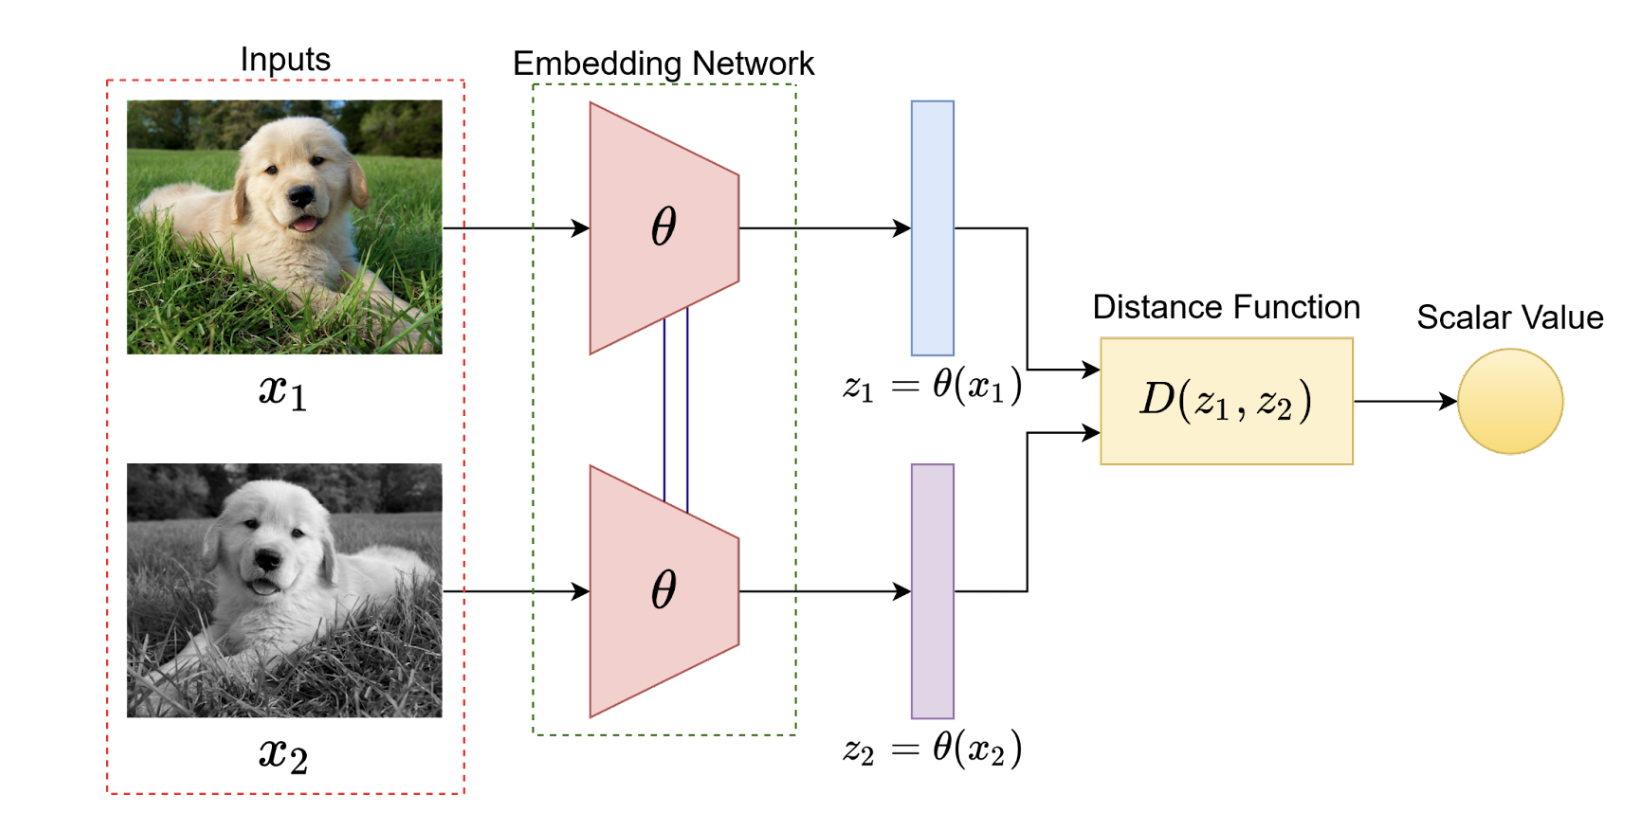
\includegraphics[width=10cm]{dog1.png}
	\captionsetup{font=small} % Adjust the font size of the caption
	\caption{معماری تعبیه مشترک}
	\label{fig:self1}
\end{figure}

\subsection{ الگوریتم‌های متضاد}

الگوریتم‌های متضاد  \LTRfootnote{\lr{Contrastive learning}}‌ با مقایسه و تضاد دیدگاه‌های مختلف از یک داده کار می‌کنند. این مدل آموزش داده شده است تا نقاط داده مشابه را در فضای بازنمایی آموخته شده به هم نزدیک کند در حالی که نقاط داده غیرمشابه را از هم جدا کند. 
%یادگیری متضاد می تواند از فراوانی نمونه های منفی بهره مند شود که به بهبود استحکام مدل کمک می کند.
%این الگوریتم‌ها نیازی به مدل‌سازی مولد صریح ندارند و می‌توانند از نظر محاسباتی کارآمدتر باشند.
هدف الگوریتم‌های متضاد، تضاد دیدگاه‌های مختلف از داده‌های مشابه برای یادگیری نمایش‌های معنادار است. آنها جفت‌های مثبت و منفی نمونه‌های داده را ایجاد می‌کنند و مدل را تشویق می‌کنند تا نمونه‌های مشابه را نزدیک‌تر کند در حالی که نمونه‌های غیرمشابه را در فضای نمایش آموخته‌شده از هم جدا می‌کنند. 
\citep{liu2021self}
در شکل  \ref{fig:self2} دو نمونه از داده مربوط به تصویر سگ به عنوان نمونه مشابه و یک تصویر گربه به عنوان نمونه غیر مشابه در فضای برداری نشان داده شده است که مدل یادگیری متضاد سعی ‌می‌کند فاصله نمونه‌های مشابه را به حداقل و فاصله نمونه‌های غیر مشابه را به حداکثر در فضای برداری برساند.
\citep{falcon2020framework}
% \begin{figure}[htbp]
%	\centering
%	
%\end{figure}

\begin{minipage}{\linewidth}
	\centering
	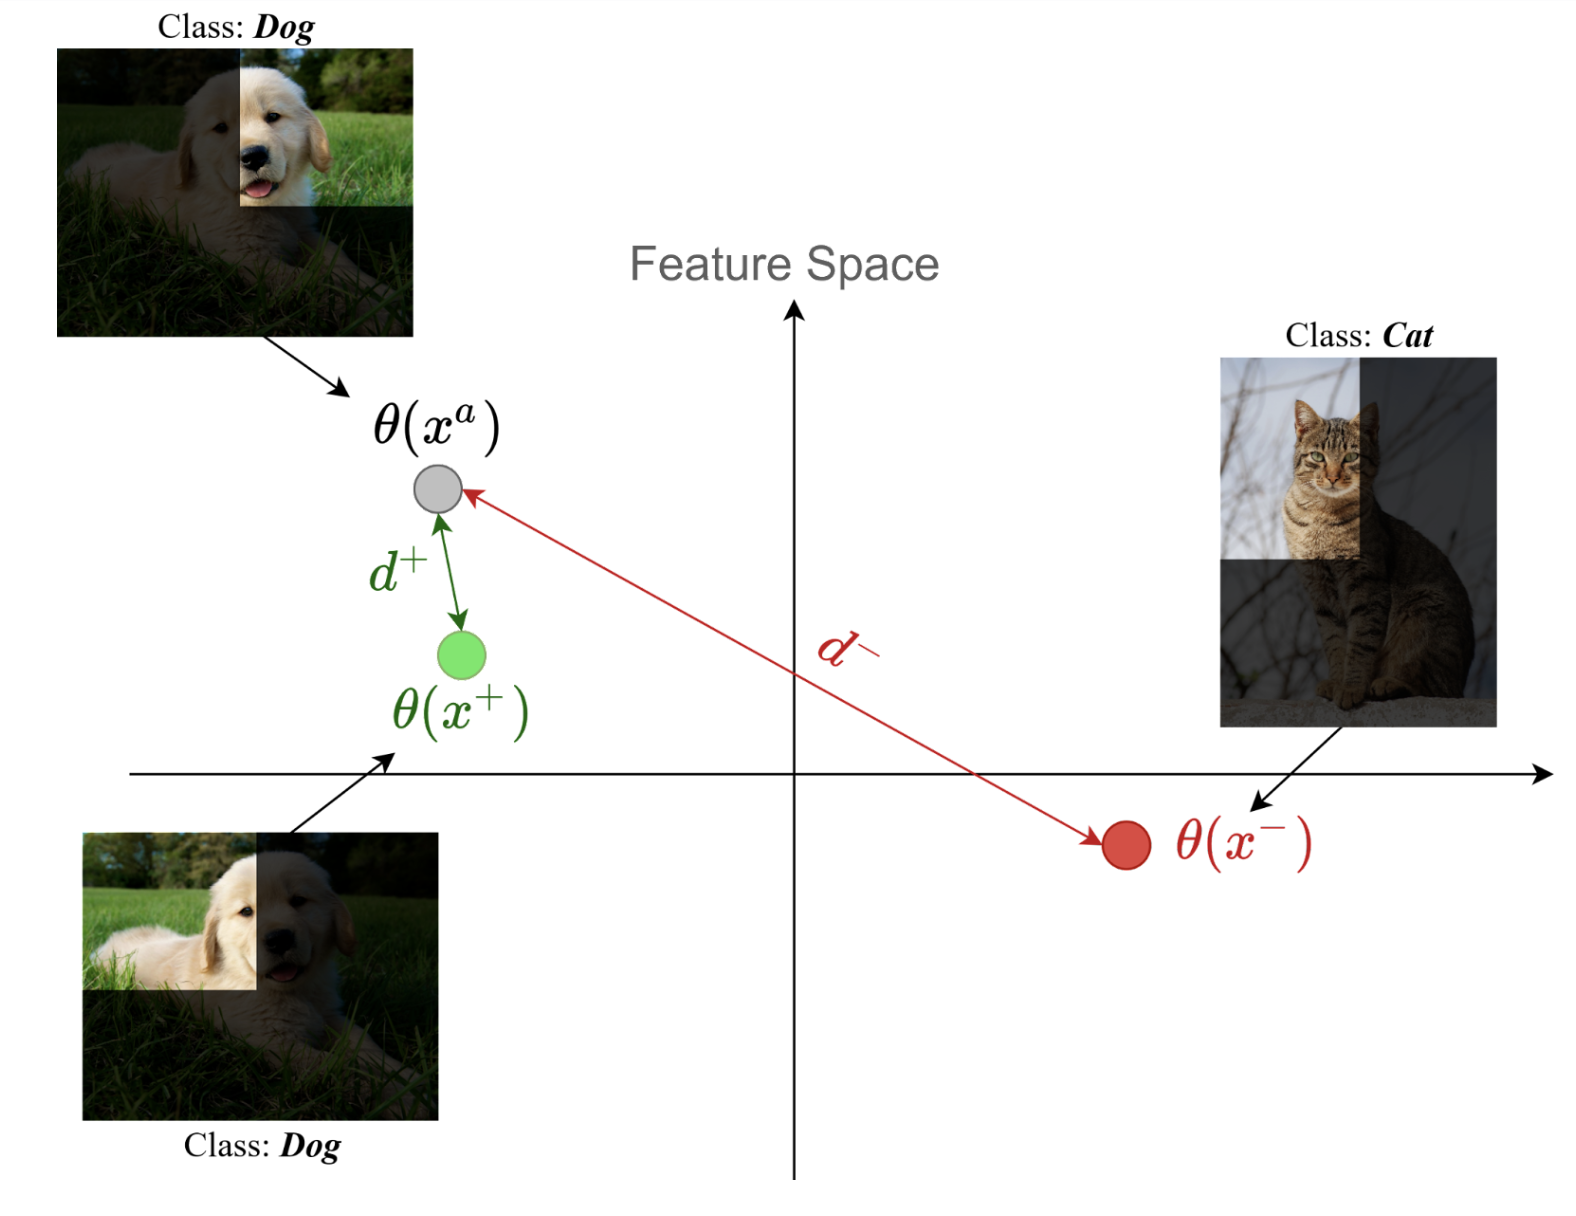
\includegraphics[width=10cm]{dog2.png}
	\captionsetup{font=small} % Adjust the font size of the caption
	\captionof{figure}{الگوریتم یادگیری متضاد}
	\label{fig:self2}
\end{minipage}



\subsection{ روش های تبعیض نمونه}

روش‌های تبعیض نمونه \LTRfootnote{\lr{Instance discrimination method}}‌از ایده کلی یادگیری متضاد، برای کل نمونه‌های داده (مانند یک تصویر کامل) استفاده می کنند.

به عنوان مثال، دو نسخه چرخانده یا برگردان شده از یک تصویر سگ می‌توانند به عنوان جفت  مثبت عمل کنند، در حالی که یک نسخه چرخانده/برگردان شده از یک تصویر گربه می‌تواند به عنوان نمونه منفی باشد. اکنون، مشابه اصل اساسی، فاصله بین جفت مثبت باید به حداقل برسد، در حالی که فاصله بین جفت منفی باید حداکثر شود.

ایده اصلی پشت این تکنیک این است که ورودی, که دستخوش برخی تبدیل‌های داده‌های اساسی شده است باید همچنان از همان دسته باشد، یعنی یک مدل یادگیری عمیق باید نسبت به تبدیل‌ها تغییر ناپذیر باشد. هنگامی که تصویر یک سگ به صورت عمودی چرخانده می‌شود و به مقیاس خاکستری تبدیل می‌شود، همچنان کلاس "سگ" را نشان می دهد.
\citep{taher2022caid}
در این دسته از روش‌ها، یک تصویر تصادفی گرفته می‌شود و تبدیل تصادفی برای ایجاد نمونه مثبت روی آن اعمال می شود (مانند چرخش، برش و غیره). اکنون، چندین تصویر دیگر از مجموعه داده به عنوان نمونه‌های منفی گرفته می شود و یک تابع هزینه طراحی شده است تا فاصله بین جفت‌های نمونه منفی را به حداکثر برساند. شکل \ref{fig:self3}

\begin{minipage}{\linewidth}
	\centering
	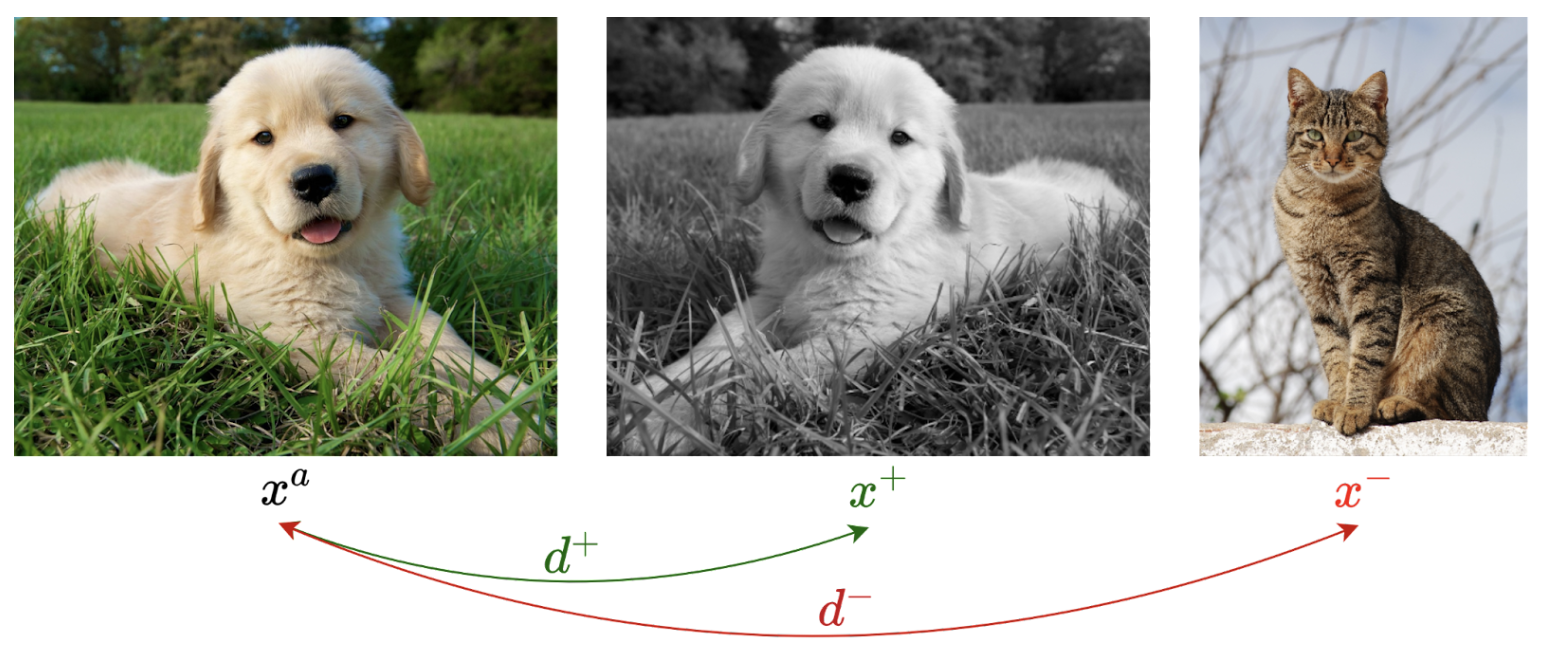
\includegraphics[width=10cm]{dog3.png}
	\captionsetup{font=small} % Adjust the font size of the caption
	\captionof{figure}{روش‌های تبعیض نمونه}
	\label{fig:self3}
\end{minipage}

یکی از روش‌های محبوب در دسته روش‌های تبعیض نمونه الگوریتم یادگیری متضاد ساده\LTRfootnote{\lr{Simplified contrastive learning(simclr)}})  است که در ادامه به توضیح این روش می‌پردازیم


\subsubsection{SimCLR (یادگیری متضاد ساده)}


یک روش یادگیری خود نظارت برای تصاویری است که از یادگیری متضاد برای یادگیری نمایش داده‌ها بدون تکیه بر داده‌های برچسب‌گذاری شده استفاده می‌کنند. این شامل آموزش یک شبکه عصبی برای پیش‌بینی این است که کدام دو تصویر، از یک جفت تصویر، شبیه‌تر هستند. نمایش‌هایی که شبکه یاد می‌گیرد می‌تواند به عنوان جاسازی ویژگی برای کارهای پایین دستی مانند دسته‌بندی تصویر استفاده شود.
\citep{falcon2020framework}
%SimCLR یک چارچوب یادگیری خود نظارت است که توسط Google Research پیشنهاد شده است. این برای یادگیری بازنمایی های بصری قدرتمند با استفاده از یادگیری متضاد طراحی شده است. ایده اصلی پشت SimCLR این است که جفت نماهای تقویت شده مثبت و منفی را از یک نمونه داده ایجاد کند و سپس آنها را در فضای نمایش آموخته شده مقایسه کند.
روش یادگیری متضاد ساده از اجزای کلیدی زیر تشکیل شده است:

1.افزایش داده‌ها\LTRfootnote{\lr{Data augmentation}} : 

هر نمونه ورودی دو بار افزوده می‌شود تا دو نمای متفاوت از یک نقطه داده ایجاد شود.

2.شبکه رمزگذار \LTRfootnote{\lr{Encoder}} : 

یک شبکه عصبی (معمولاً یک شبکه عصبی پیچشی عمیق) برای استخراج ویژگی از نماهای تقویت‌شده داده استفاده می‌شود.

3.سر نمایش دهنده  \LTRfootnote{\lr{Projection head}} :

یک پرسپترون چندلایه \LTRfootnote{\lr{Multilayer preceptron}} با یک لایه پنهان است که فقط بردارهای نمایش را قبل از تابع هزینه کوچک‌تر می‌کند.

4.تابع هزینه متضاد\LTRfootnote{\lr{Contrastive loss function}} : 

هدف مدل این است که نمایش‌های جفت‌های مثبت (نماهای تقویت‌شده همان نمونه) را نزدیک‌تر کند و نمایش‌های جفت‌های منفی (نماهای تقویت‌شده نمونه‌های مختلف) را در فضای ویژگی دورتر کند. تابع هزینه متضاد مدل را تشویق می‌کند تا بازنمایی‌های متمایزکننده‌ای را بیاموزد که ویژگی‌های اساسی داده‌ها را ضبط می‌کند.

در شکل  \ref{fig:self4}  روند کلی الگوریتم یادگیری متضاد ساده نشان داده شده است به این صورت که دو داده افزوده شده به شبکه داده می‌شود و شبکه می آموزد نمایش داده های مربوط به یک کلاس را مشابه هم و نمایش داده‌های کلاس‌های مختلف را متفاوت تولید کند.

\begin{minipage}{\linewidth}
	\centering
	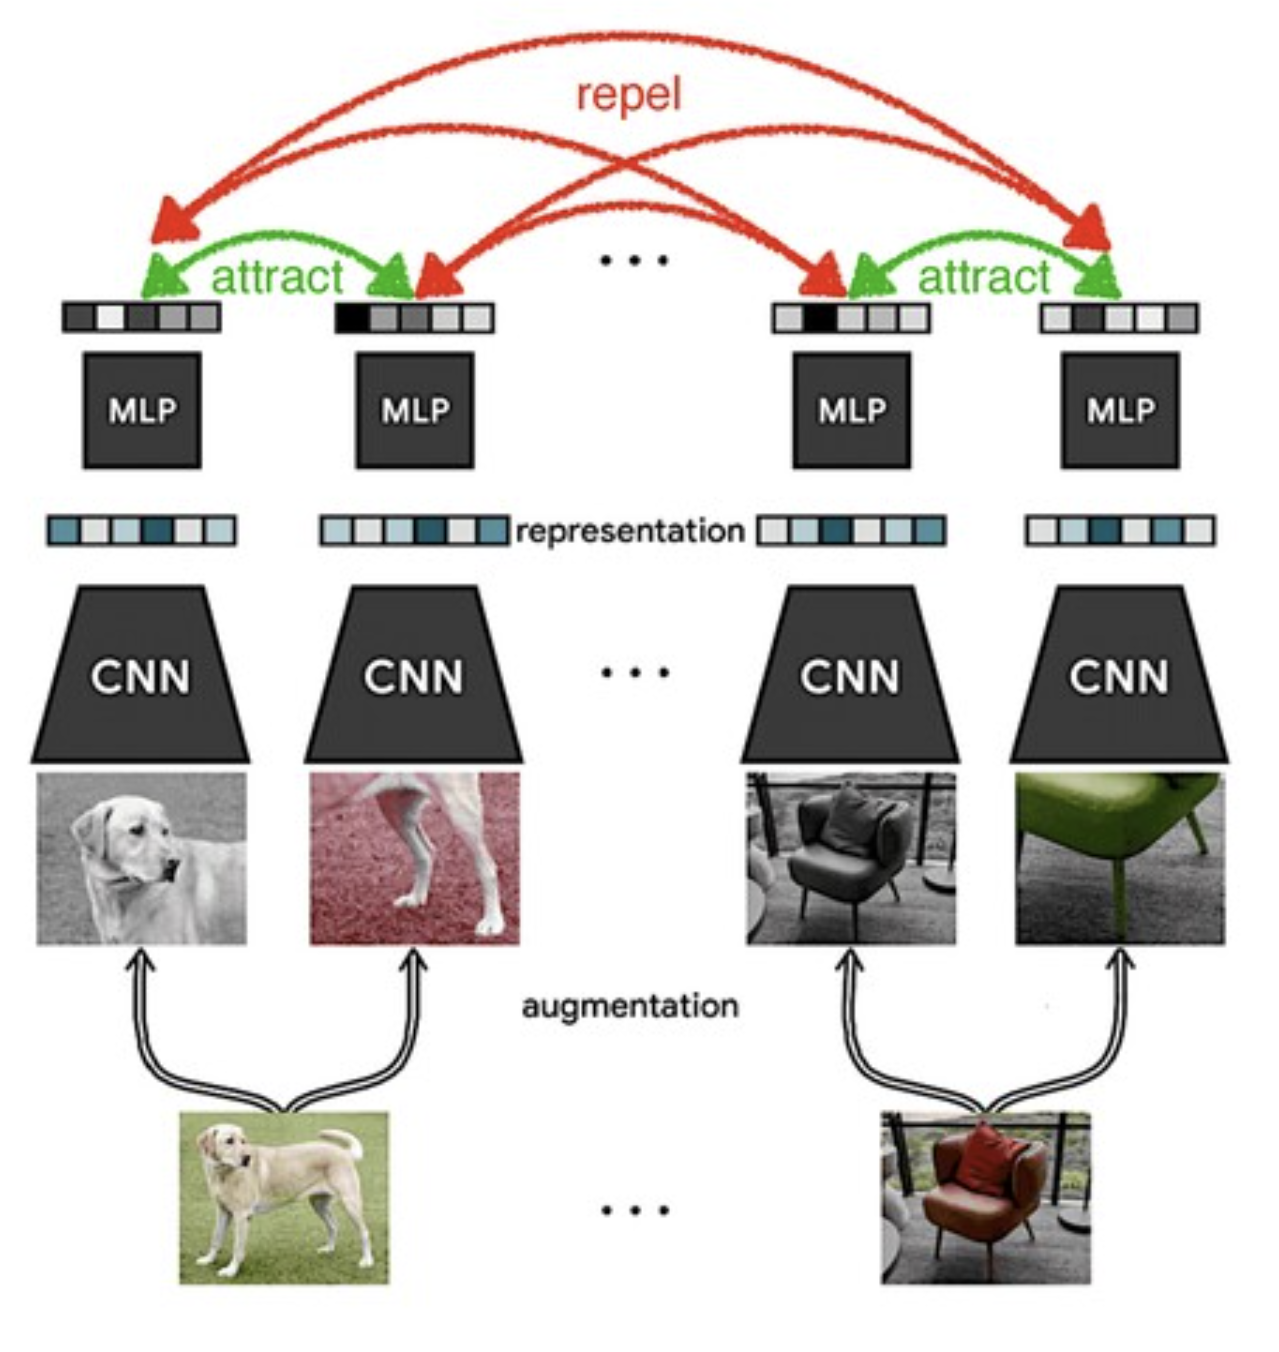
\includegraphics[width=10cm]{dog4.png}
	\captionsetup{font=small} % Adjust the font size of the caption
	\captionof{figure}{روش یادگیری متضاد ساده}
	\label{fig:self4}
\end{minipage}

%\subsubsection{MoCo (مقابل حافظه تقویت شده)}
%MoCo یکی دیگر از چارچوب های یادگیری تحت نظارت خود است که توسط محققان در فیس بوک AI Research (FAIR) معرفی شده است. این نیاز به بانک های حافظه بزرگ برای رسیدگی به تعداد زیادی از نمونه های منفی را برطرف می کند، محدودیتی که الگوریتم های متضاد قبلی با آن مواجه بودند. MoCo از یک بافر حافظه برای ذخیره فرهنگ لغت بزرگی از تعبیه‌های ویژگی استفاده می‌کند که امکان یادگیری متضاد کارآمد با تعداد زیادی نگاتیو را فراهم می‌کند.
%اجزای کلیدی MoCo عبارتند از:
%
%Momentum Update: MoCo یک شبکه رمزگذار مومنتوم را معرفی می کند که میانگین متحرک وزن رمزگذار اصلی است. این امکان نمایش ویژگی های پایدارتر و موثرتر را فراهم می کند.
%Memory Queue: یک بافر حافظه مبتنی بر صف، نمایش نمونه های منفی را ذخیره می کند. در طول آموزش، خروجی رمزگذار در حافظه قرار می‌گیرد و قدیمی‌ترین عناصر صف حذف می‌شوند. این مدل را قادر می سازد تا مجموعه بزرگ و متنوعی از نمونه های منفی را بدون ذخیره صریح آنها حفظ کند.
%هر دو SimCLR و MoCo عملکرد چشمگیری را در وظایف مختلف بینایی کامپیوتری مانند طبقه بندی تصویر، تشخیص اشیا و تقسیم بندی نشان داده اند. این الگوریتم‌های متضاد به طور قابل‌توجهی زمینه یادگیری خود نظارتی را ارتقا داده‌اند و بینش‌های ارزشمندی را برای یادگیری نمایش‌های قدرتمند از داده‌های بدون برچسب به شیوه‌ای بدون نظارت ارائه می‌دهند.

%3. روش های مبتنی بر رمزگذار خودکار:
%رمزگذارهای خودکار شبکه های عصبی هستند که برای بازسازی داده های ورودی از یک نمایش با ابعاد پایین تر (رمزگذار) و سپس بازسازی آن به شکل اصلی (رمزگشا) آموزش دیده اند. رمزگذارهای خودکار با نظارت خود با به حداقل رساندن خطای بازسازی، نمایش های مفیدی را یاد می گیرند.
%
%4. پیش بینی چرخش:
%این روش شامل آموزش مدل برای پیش بینی زاویه چرخش یک تصویر است. با انجام این کار، مدل یاد می‌گیرد که تغییر ناپذیری چرخشی و ویژگی‌های معنادار را ثبت کند.
%
%5. پیش بینی زمینه:
%پیش‌بینی زمینه شامل آموزش مدل برای پیش‌بینی بخش‌های گمشده یا زمینه یک تصویر، اغلب با حذف تکه‌ها یا پوشاندن تصادفی بخش‌هایی از تصویر ورودی است.
%
%6. نمونه تبعیض:
%در این رویکرد، مدل یاد می‌گیرد که با در نظر گرفتن تکنیک‌های افزایش داده‌ها برای ایجاد تغییرات نمونه، بین نمونه‌های مختلف یک کلاس یا شی تمایز قائل شود.

%7. پازل های اره منبت کاری اره مویی:
%پازل‌های اره منبت کاری اره مویی شامل شکستن یک تصویر به چند تکه و به هم ریختن آن‌ها هستند و مدل آموزش داده می‌شود تا با چیدمان صحیح وصله‌ها، معما را حل کند.
%
%8. پیش بینی ترتیب زمانی:
%این روش برای داده های متوالی مانند ویدئو یا صدا استفاده می شود. این مدل برای پیش‌بینی ترتیب زمانی صحیح فریم‌های به هم ریخته یا بخش‌های صوتی آموزش داده شده است.
%
%9. انتساب خوشه:
%انتساب خوشه شامل خوشه بندی نقاط داده در فضای نمایش آموخته شده، تشویق مدل به یادگیری جداسازی موثر خوشه های مختلف است.
%
%اینها تنها نمونه هایی از طیف متنوع الگوریتم های مورد استفاده در یادگیری خود نظارت هستند. هر الگوریتم با چالش ایجاد سیگنال‌های نظارت معنی‌دار از داده‌های بدون برچسب به روش‌های منحصربه‌فردی مقابله می‌کند و کاربردهای آن‌ها به حوزه‌های مختلفی از جمله بینایی رایانه، پردازش زبان طبیعی و تشخیص گفتار گسترش می‌یابد.



\section{روش های افزایش داده و تولید نمونه های جدید}

افزایش داده‌ها \LTRfootnote{\lr{Data augmentation}}یک تکنیک مهم در حوزه یادگیری ماشین است که با استفاده از تغییرات مختلف بر روی داده‌های اصلی، حجم و تنوع مجموعه آموزشی را افزایش می‌دهد. هدف اصلی این تکنیک، کاهش اهمیت بار آموزشی و جلوگیری از بیش‌برازش مدل‌ها به داده‌های آموزشی است. با افزایش تنوع داده‌ها، مدل‌های یادگیری ماشین قادر به بهترین فراگیری الگوها و ویژگی‌ها می‌شوند و در مواجهه با داده‌های جدید و ناشناخته، عملکرد بهتری از خود نشان می‌دهند.
\citep{ng2020ssmba}
افزایش داده‌ها از روش‌های متنوعی مانند تغییرات هندسی، تبدیل‌های رنگی، برش‌ها و چرخش‌ها، نویز اضافه کردن به داده‌ها و... استفاده می‌کند. با اعمال این تغییرات، داده‌ها به شکل مصنوعی تغییر می‌کنند و مجموعه آموزشی با داده‌های جدید و تا حدودی ناشناخته تکمیل می‌شود. این تغییرات همچنین باعث افزایش دقت و پایداری مدل‌ها در مواجهه با شرایط مختلفی می‌شود که ممکن است در داده‌های ورودی واقعی وجود داشته باشند.

در انجام افزایش داده‌ها، اهمیت استفاده از روش‌های مناسب و متعادل برای تغییر داده‌ها وجود دارد. از یک سو، باید مطمئن شویم که داده‌های تغییر یافته معتبر و معنادار هستند و با ویژگی‌های داده‌های اصلی همخوانی دارند. از سوی دیگر، تغییرات اعمال شده نباید اطلاعات اصلی و اساسی داده‌ها را به طور قابل ملاحظه‌ای تغییر دهد تا از از دست دادن اطلاعات مهم جلوگیری شود. به کارگیری تکنیک‌های افزایش داده‌ها باعث بهبود عملکرد و کارایی مدل‌های یادگیری ماشین در حل مسائل مختلف می‌شود و در عمل، جزء مهمی از روش‌های موفق در حوزه یادگیری ماشین به شمار می‌آید.

افزایش داده‌ها  یکی از روش‌های موثر در بهبود عملکرد مدل‌های یادگیری ماشین است. کتابخانه PyTorch ابزارهای متنوعی برای انجام افزایش داده‌ها فراهم می‌کند که به ما اجازه می‌دهد داده‌ها را به صورت مصنوعی تغییر داده و تنوع آن‌ها را افزایش دهیم. در ادامه، به برخی از روش‌های افزایش داده‌ها در PyTorch پرداخته می‌شود:

۱. تغییرات هندسی: این روش‌ها شامل تغییر اندازه، برش، چرخش و انعکاس داده‌ها است. با اعمال این تغییرات، می‌توانیم داده‌ها را به صورت مختلف در فضای هندسی قرار دهیم و از این طریق تنوع مجموعه آموزشی را افزایش دهیم.

۲. تبدیل‌های رنگی: این روش‌ها شامل تغییر رنگ، کنتراست و روشنایی تصاویر است. با اعمال تبدیل‌های رنگی، می‌توانیم داده‌ها را به صورت مصنوعی تغییر رنگ دهیم و با ایجاد تصاویر مختلف، مجموعه آموزشی را متنوع‌ کنیم.

۳. افزودن نویز: با افزودن نویز به داده‌ها، می‌توانیم شباهت آن‌ها را کاهش داده و مدل‌ها را در برابر داده‌های جدید و ناشناخته آماده کنیم. افزودن نویز به تصاویر و ویدئوها از جمله روش‌های متداول این دسته است.


در شکل \ref{fig:self5} نمونه‌هایی از اعمال روش‌های مختلف افزایش داده نشان داده شده است که همانطور که گفته شد برای پیاده سازی الگوریتم‌های یادگیری خودنظارتی به این تکنیک‌های افزایش  داده نیازمند هستیم.

\begin{minipage}{\linewidth}
	\centering
	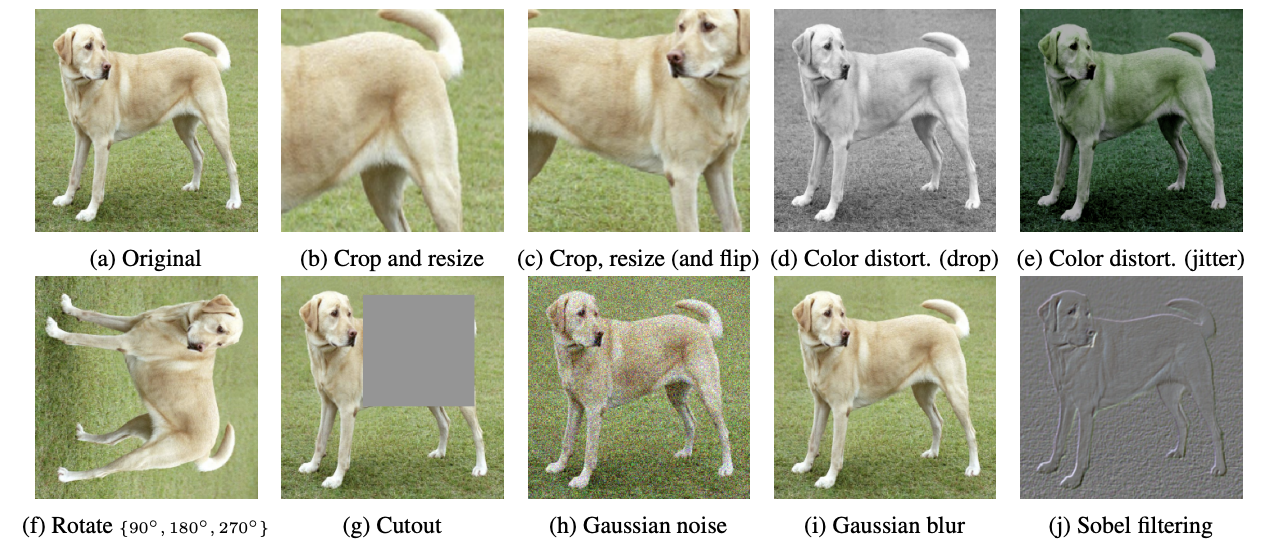
\includegraphics[width=12cm]{dog5.png}
	\captionsetup{font=small} % Adjust the font size of the caption
	\captionof{figure}{روش‌های افزایش داده}
	\label{fig:self5}
\end{minipage}


\section{مفهوم انتقال یادگیری در یادگیری خود نظارتی}

انتقال یادگیری \LTRfootnote{\lr{Transfer learning}} یکی از روش‌های مؤثر در یادگیری خودنظارتی است که به کمک آن می‌توان اطلاعات آموزش‌دیده شده از یک مسئله را به مسئله‌ی دیگری منتقل کرد. در یادگیری خودنظارتی، معمولاً از اطلاعات بدون نظارت در داده‌ها برای آموزش مدل‌ها استفاده می‌شود. اما با انتقال یادگیری، می‌توان از اطلاعات آموزش‌دیده شده در یک مسئله برای حل مسئله‌ی دیگری بهره‌برداری کرد. در شکل \ref{fig:self6} مفهوم انتقال یادگیری در یادگیری ماشین در مقایسه با یادگیری ساده نشان داده شده است.

\begin{minipage}{\linewidth}
	\centering
	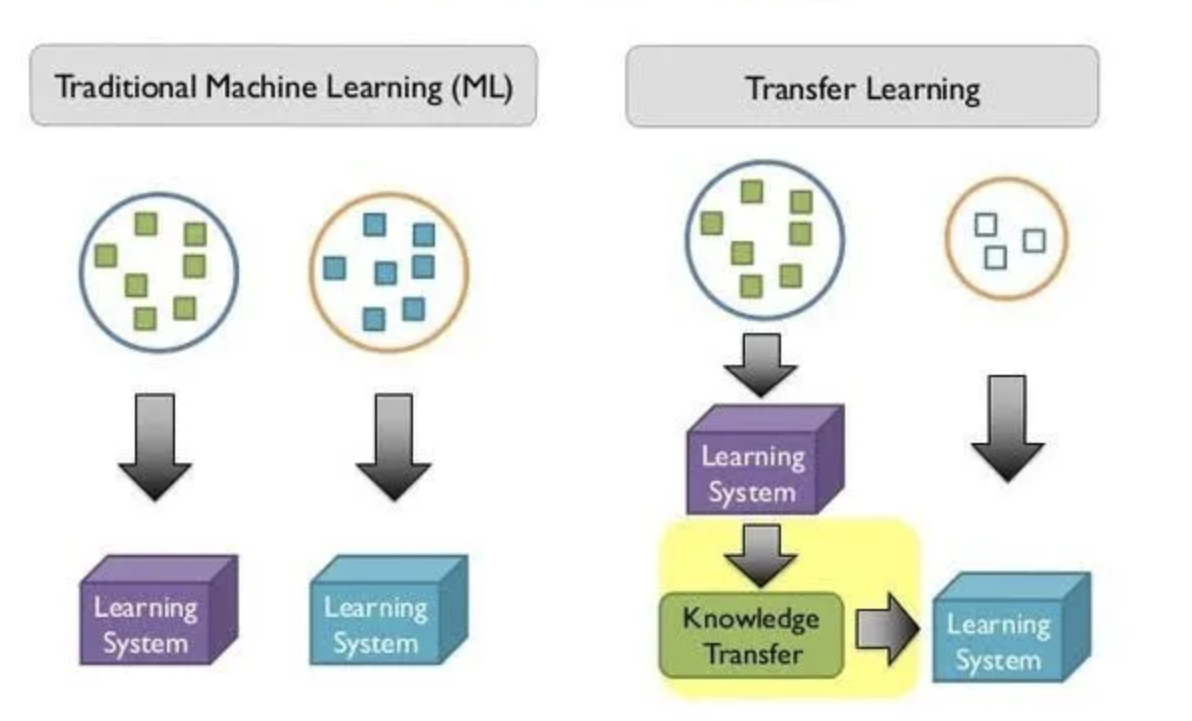
\includegraphics[width=10cm]{self1.png}
	\captionsetup{font=small} % Adjust the font size of the caption
	\captionof{figure}{انتقال یادگیری در مقایسه با یادگیری ساده}
	\label{fig:self6}
\end{minipage}

یکی از روش‌های معمول استفاده از انتقال یادگیری در یادگیری خودنظارتی، استفاده از مدل‌های پیش‌آموزش‌دیده \LTRfootnote{\lr{ Pre-trained models}} است. در این روش، یک مدل با داده‌های بدون برچسب آموزش داده می‌شود. سپس وزن‌های این مدل به عنوان وزن‌های اولیه در حل مسئله‌ی هدف استفاده می‌شود. این انتقال وزن‌ها امکان دسترسی به اطلاعات بدون نظارت از داده‌های پیشین و بهره‌گیری از آن‌ها برای بهبود عملکرد مدل را فراهم می‌کند.
\citep{mao2020survey}
همچنین در انتقال یادگیری در یادگیری خودنظارتی، می‌توان از لایه‌های مشترک میان دو مسئله استفاده کرد. این لایه‌های مشترک می‌توانند اطلاعات کلیدی را که در هر دو مسئله به کار می‌روند، از داده‌های پیشین یاد بگیرند و از آن‌ها برای حل مسئله‌ی هدف استفاده کنند. این روش از نظر محدودیت داده‌ها و منابع محاسباتی مؤثر است و می‌تواند عملکرد مدل‌ها را بهبود بخشد.



تمایز اصلی انتقال یادگیری از یادگیری معمولی این است که در انتقال یادگیری، مدل از داده‌ها و دانش موجود در یک مسئله به مسئله‌ی دیگری منتقل می‌شود. این روش بسیار مؤثر در مواردی است که داده‌های کافی برای آموزش مدل در مسئله‌ی هدف موجود نیست یا هزینه‌ی جمع‌آوری داده‌های جدید بسیار بالاست.

انتقال یادگیری در حوزه‌های مختلفی از جمله بینایی ماشین، پردازش زبان طبیعی، تشخیص الگو و بازیابی اطلاعات استفاده می‌شود و به دلیل کارایی و عملکرد بالا، از محبوبیت بسیاری برخوردار است.
استفاده از انتقال یادگیری در یادگیری خودنظارتی باعث افزایش سرعت آموزش مدل‌ها، بهبود کیفیت نتایج و کاهش نیاز به داده‌های برچسب‌دار می‌شود. در این روش شبکه ابتدا با داده‌های اولیه \LTRfootnote{\lr{Pretext}}بدون برچسب  آموزش می‌بیند سپس شبکه آموزش دیده شده برای حل مساله اصلی با داده‌های برچسب دار استفاده می شود. در شکل \ref{fig:self7} ابتدا شبکه بر روی داده‌های بدون برچسب آموزش می‌بیند و یک نمایش از داده‌ها تولید می‌کند سپس شبکه آموزش دیده شده برای حل یک مساله نظارت شده استفاده می‌شود و در طی یادگیری بر روی داده‌های جدید برچسب دار به  جای از ابتدا آموزش دیدن صرفا تنظیم دقیق \LTRfootnote{\lr{Finetune}}می شود که بسیار سریع و بهینه است.
\citep{medina2020self}

\begin{minipage}{\linewidth}
	\centering
	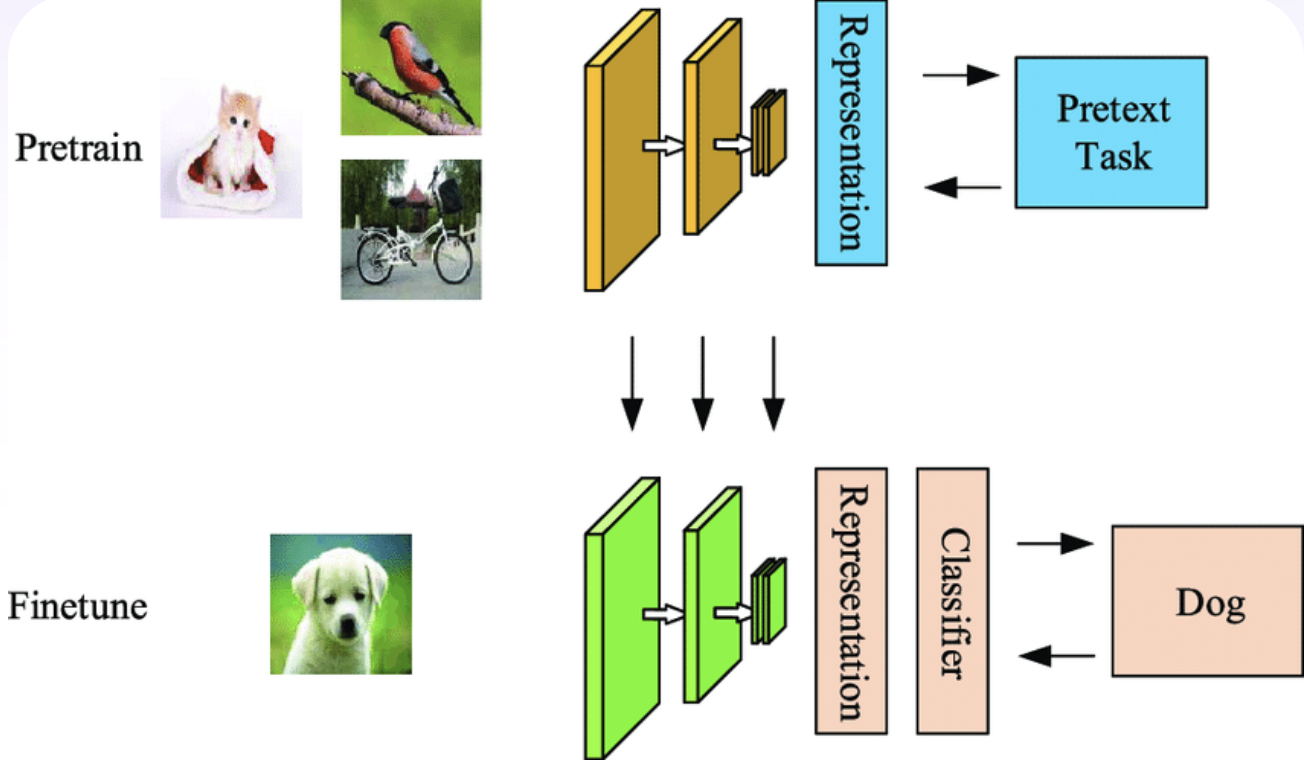
\includegraphics[width=10cm]{self7.png}
	\captionsetup{font=small} % Adjust the font size of the caption
	\captionof{figure}{انتقال یادگیری در فرایند یادگیری خودنظارتی}
	\label{fig:self7}
\end{minipage}


\section{ توابع هزینه در یادگیری خودنظارتی}

در یادگیری خودنظارتی متضاد، تابع خطای مقایسه‌ای برای آموزش مدل به کار می‌رود. هدف اصلی این تابع خطا، ایجاد فضای نمونه در مدل است که نمونه‌های مشابه در این فضا به هم نزدیک شوند، در حالی که نمونه‌های متفاوت از یکدیگر فاصله داشته باشند. با ایجاد این فضای نهان، مدل حساس به تفاوت‌های بین داده‌ها می‌شود و می‌تواند الگوهای مشترک بین داده‌ها را برای تمایز دادن از هم استخراج کند.
\citep{falcon2020framework}
برای تعریف تابع خطا به طور کلی از تابع هزینه رتبه بندی حاشیه  \LTRfootnote{\lr{Margin ranking}}استفاده می‌شود. در این روش، برای هر نمونه اصلی، دو نمونه دیگر انتخاب می‌شوند: یک نمونه مثبت (که مشابه نمونه‌ی اصلی است) و یک نمونه منفی (که با نمونه‌ی اصلی تفاوت دارد). سپس فاصله‌ی نمونه‌ی مثبت از نمونه‌ی اصلی (به عنوان فاصله مثبت) و فاصله‌ی نمونه‌ی منفی از نمونه‌ی اصلی (به عنوان فاصله منفی) محاسبه می‌شود. هدف این تابع خطا، مطمئن شدن از اینکه فاصله‌ی مثبت کمتر از فاصله‌ی منفی باشد و یک حداقل فاصله بین آن‌ها به عنوان لبه وجود داشته باشد. اگر فاصله‌ی مثبت از فاصله‌ی منفی بزرگتر از لبه باشد، تابع خطا مقدار آن را کاهش می‌دهد، در غیر این صورت،  تابع خطا مقدار را افزایش می‌دهد.

در تعریف تابع خطای مقایسه‌ای، می‌توان از انواع مختلفی از فاصله‌ها استفاده کرد، از جمله فاصله اقلیدسی و یا شباهت کسینوسی. همچنین می‌توان مقدار فاصله لبه و انتخاب نمونه‌های مثبت و منفی را به طور دلخواه تنظیم کرد تا بهترین نتایج را بدست آورد.

با استفاده از تابع خطای مقایسه‌ای در یادگیری خودنظارتی متضاد، مدل قادر به استخراج ویژگی‌های معنادار از داده‌ها و یادگیری نمایشی مناسب برای مسائل مختلف خواهد بود. این تابع خطا می‌تواند برای مسائل تشخیص الگو، دسته‌بندی و مدل‌سازی مقایسه‌ای داده‌ها با موفقیت استفاده شود.
\citep{jiao2022timeautoad}
از میان تابع‌های هزینه خودنظارتی، سه تابع رایج عبارتند از:

1. تابع هزینه مقایسه‌ای  \LTRfootnote{\lr{Contrastive Loss}}: 
این تابع برای مسائل مدل‌سازی از نظر مشابهت داده‌ها به کار می‌رود. در این روش، دو نمونه از یک دسته به عنوان ورودی به مدل داده می‌شوند و مدل باید بتواند دو نمونه مشابه را از یکدیگر تشخیص دهد. اگر دو نمونه متفاوت باشند، مدل باید بتواند بین آن‌ها تفاوت را تشخیص دهد. یک فاصله برای لبه در نظر گرفته می شود و با استفاده از محاسبه فاصله اقلیدسی بین نمونه‌های مشابه و غیر مشابه تابع هزینه به صورت زیر تعریف می‌شود :

%\begin{minipage}{\linewidth}
%	\centering
%	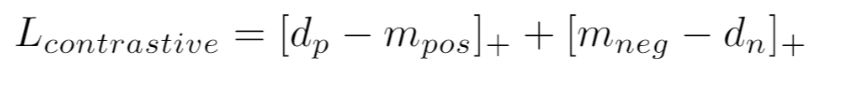
\includegraphics[width=10cm]{loss1.png}
%	%\captionof{figure}{انتقال یادگیری در مقایسه در فرایند یادگیری خودنظارتی}
%	%\label{fig:self7}
%\end{minipage}

\begin{equation}
\mathcal{L}_{\text{contrastive}} = [\text{d}_\text{positive} - \text{m}_\text{positive}] + [\text{m}_\text{negative} - \text{d}_\text{negative}]
\end{equation}




2. تابع هزینه آنتروپی متقاطع با مقیاس دمایی نرمال شده \LTRfootnote{\lr{Normalized Temperature-scaled Cross Entropy }} این تابع برای مسائل تشخیص الگو و مدل‌سازی مقایسه‌ای داده‌ها مورد استفاده قرار می‌گیرد. در این روش، نمونه‌های مختلف از یک دسته با هم مقایسه می‌شوند و مدل باید بتواند نمونه‌های مشابه را از دیگر نمونه‌ها تمایز دهد. تابع ابتدا شباهت کسینوسی یک جفت داده مثبت را محاسبه کرده و سپس آن را تقسیم بر همین مقدار برای کل جفت‌های مثبت در آن دسته داده ‌می‌کند.
\citep{falcon2020framework}

\begin{equation}
	\mathcal{L}_{\text{NTXent}} = -\frac{1}{N} \sum_{i=1}^{N} \log \frac{\exp(\text{sim}(z_i, z_{\text{pos}}) / \tau)}{\sum_{j=1}^{2N} \exp(\text{sim}(z_i, z_j) / \tau)}
\end{equation}


3. تابع هزینه سه‌قلو  \LTRfootnote{\lr{Triplet loss}}: 
این تابع برای مسائل دسته‌بندی و مدل‌سازی مقایسه‌ای داده‌ها مورد استفاده قرار می‌گیرد. به طور کلی مشابه تابع هزینه مقایسه‌ای رفتار می‌کند با این تفاوت که در این روش، سه نمونه از یک دسته به عنوان ورودی به مدل داده می‌شوند: یک نمونه مثبت (که مشابه نمونه‌ی اصلی است)، یک نمونه منفی (که با نمونه‌ی اصلی تفاوت دارد) و نمونه‌ی اصلی. مدل باید بتواند نمونه‌های مشابه را از دیگر نمونه‌ها تمایز دهد و از نمونه منفی فاصله بگیرد. فاصله نمونه‌های مثبت باید برای تمامی نمونه‌ها حداقلی باشد تا مدل به طور کلی درک درستی از دسته‌ها داشته باشد. تابع هزینه سه‌قلو معمولاً از فاصله اقلیدسی یا شباهت کسینوسی رای محاسبه فاصله‌ها استفاده می‌کند. در شکل  \ref{fig:self8}  نحوه محاسبه و عملکرد این تابع هزینه نشان داده‌شده‌است.
\citep{li2022tribyol}
%\begin{minipage}{\linewidth}
%	\centering
%	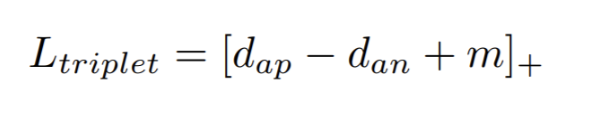
\includegraphics[width=8cm]{loss3.png}
%	%\captionof{figure}{انتقال یادگیری در مقایسه در فرایند یادگیری خودنظارتی}
%	%\label{fig:self7}
%\end{minipage}

\begin{equation}
	L = \max(d(a, p) - d(a, n) + \text{margin}, 0)
\end{equation}

\begin{minipage}{\linewidth}
	\centering
	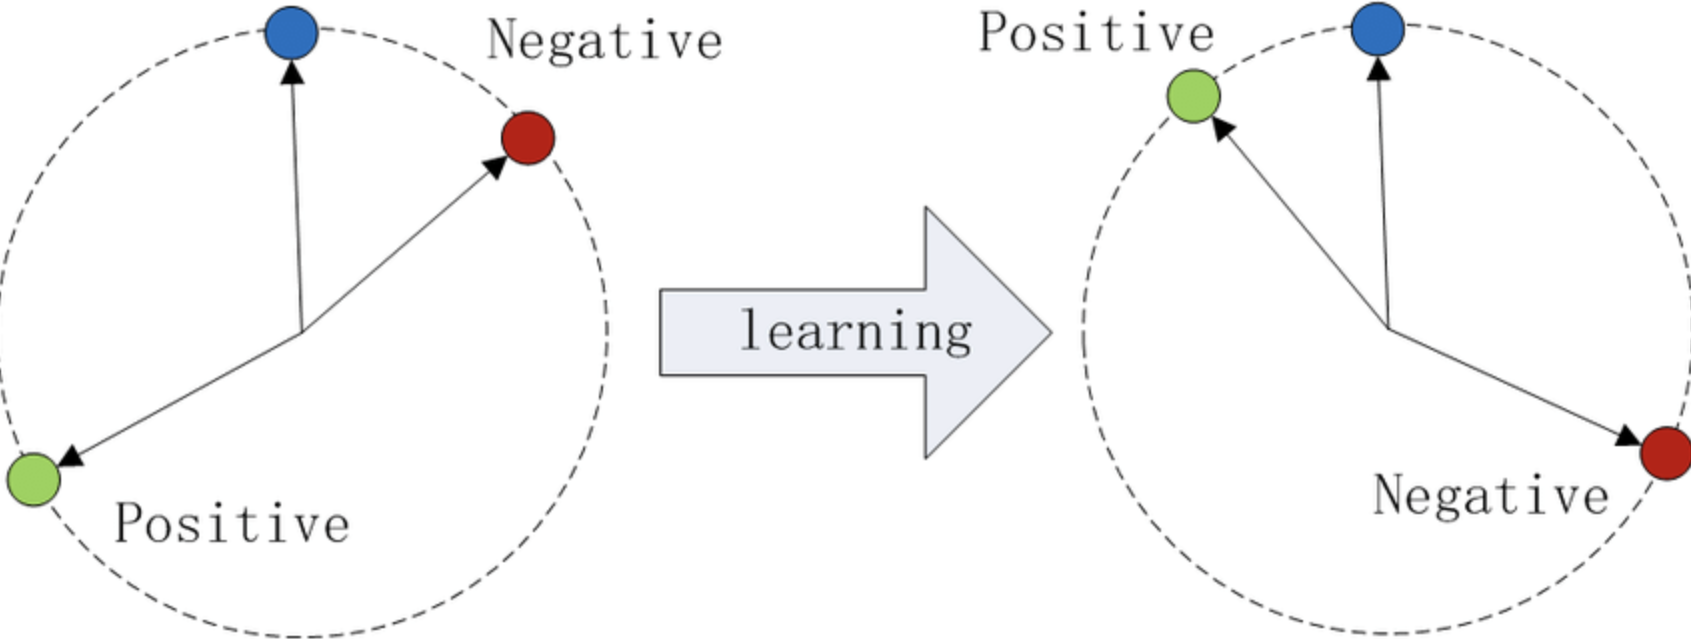
\includegraphics[width=10cm]{loss4.png}
	\captionsetup{font=small} % Adjust the font size of the caption
	\captionof{figure}{عملکرد تابع هزینه سه‌قلو }
	\label{fig:self8}
\end{minipage}


